\documentclass[output=paper]{langsci/langscibook}  
\author{%
 Christoph Rösener
\affiliation{Johannes Gutenberg University of Mainz/Germersheim}
}
\ChapterDOI{10.17169/langsci.b108.297} %will be filled in at production

\abstract{
Many research facilities and institutions contemplate the idea of setting up an eye tracking laboratory or an even more extensive usability lab of their own. However, from the initial idea to the successful implementation of such a project, there are lots of difficulties and problems, which have to be solved. Everything from room size and layout, to which technology to use, which devices to purchase and the choice of software and the methods to be used \citep{Dumas1999} -- there are many questions to answer during the conception and construction of such a laboratory. Despite this, eye tracking, as the major technique in usability research, has become more sophisticated and complex over recent years. Moreover, in usability laboratories additional equipment is needed, which in many cases has to interact with the eye tracking devices. All these are obstacles, which have to be overcome in the process of creating an eye tracking or usability laboratory. In the present paper, I will try to approach these issues from various points of view, showing the dos and don'ts in the process of setting up such a laboratory.}
\title{Eye tracking and beyond: The dos and don'ts of creating a contemporary usability lab}
\rohead{Eye tracking and beyond}
\maketitle
\begin{document}

\section{Introduction}

In this paper I will try to approach the various challenging issues one faces in planning, designing and implementing a contemporary usability lab from various points of view, showing the dos and don'ts in the process of setting up such a laboratory. Following the introduction, I will give a brief overview of modern eye tracking equipment available on the market. Several eye tracking systems are presented as well as additional devices necessary for the task. Connected with this, I shall discuss some of the main issues important for the final decision regarding which system to choose. This is then followed by a description of possible design concepts for usability laboratories in general. Finally, I will describe the difficulties and problems in using an eye tracking laboratory for usability studies. The paper ends with a presentation of the existing usability laboratory at Flensburg University of Applied Sciences and at the end some conclusions are drawn and future possibilities are discussed.


In order to get a common and clear understanding of what `usability' means, it is first of all necessary to take a closer look on the various existing definitions. Standard 9241 from the International Organization for Standardization (ISO) defines `usability' as ``[t]he effectiveness, efficiency and satisfaction with which specified users achieve specified goals in particular environments.'' \citep{ISO9241}. Effectiveness, efficiency and satisfaction are then further defined in the standard as follows: 


\begin{quote}
\textbf{effectiveness: }the accuracy and completeness with which specified users can achieve specified goals in particular environments
\end{quote}

\begin{quote}
\textbf{efficiency:} the resources expended in relation to the accuracy and completeness of goals achieved
\end{quote}

\begin{quote}
\textbf{satisfaction:} the comfort and acceptability of the work system to its users and other people affected by its use
\end{quote}

In 1992, the multi-part standard was named ``Ergonomic requirements for office work with visual display terminals''. From 2006 on, the standards were retitled to the more generic ``Ergonomics of Human System Interaction''. Nevertheless, it is obvious that the focus of this definition is clearly only usability in connection with software applications. In 1998, Jakob Nielsen gave a wider definition of usability:

\begin{quote}
Usability is the measure of the quality of the user experience when interacting with something -{}- whether a Web site, a traditional software application, or any other device the user can operate in some way or another.\footnote{ \citet{Nielsen1998}; cited in \citet{Eichinger1999}.}
\end{quote}

This definition includes, in addition to the classical software application, also `any other device', i.e. to my mind also objects, tools or any other sort of device. 

I will use this broader definition as a basis in order to develop the design of a contemporary usability lab. At the same time, I would like to point out that this definition expresses the wide range of possible research interests a contemporary usability lab can be used for. Concerning language and translation research, the most important method to investigate, for example, reading behaviour, comprehensibility of texts or translational behaviour is clearly eye tracking. Therefore, if only language and translation research are to be done, an eye tracking laboratory instead of a fully equipped usability laboratory might be sufficient.

  
\begin{figure}[t]
 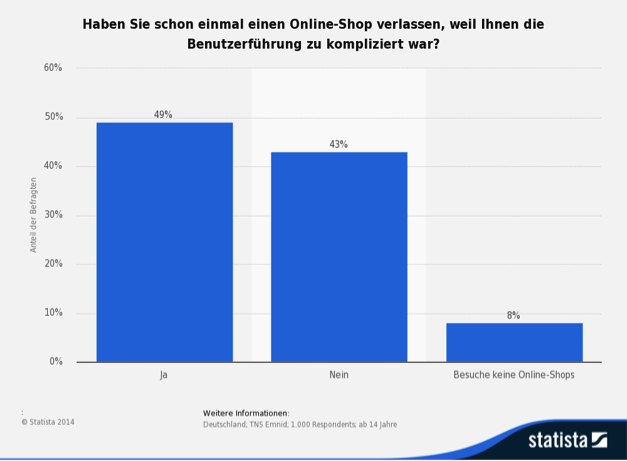
\includegraphics[width=\textwidth]{figures/Roesener1.png}
 \caption{Usability of online shops (Source: TNS Emnid 2014)}
 \label{roesener:fig:1}
\end{figure} 
 


\subsection{Motivation}

\figref{roesener:fig:1} shows the results of a survey by the German TNS Emnid opinion in 2014. 1,000 individuals of over 14 years of age were asked the question ``Have you ever left an online shop because the user interface was too difficult?''. Possible answers were ``yes'', ``no'' or ``I do not use online shops''.


From the 92\% of the web users who do use online shops, more than 50\% consider web shops too complicated sometimes. That means that more than 50\% of the web users are not satisfied with the quality and thus the usability of online shops. In contrast, in \figref{roesener:fig:2} the results of a survey concerning the use of customer-oriented instruments for online retailers are shown. The participants were asked: ``Which of the following customer-oriented instruments do you use or do you plan to use to improve the sales of your online shop?'' The given list contained the following instruments:


\begin{itemize}
\item analyzing user behaviour to identify optimization potential 
\item customer surveys to identify improvement opportunities 
\item certification by a provider of quality seals 
\item usability evaluation by external vendors 
\end{itemize}

Possible answers were ``I use this'', ``I plan to use this'' and ``Not planned''. The survey was conducted by ibi research University Regensburg GmbH. 

\begin{figure}[t]
 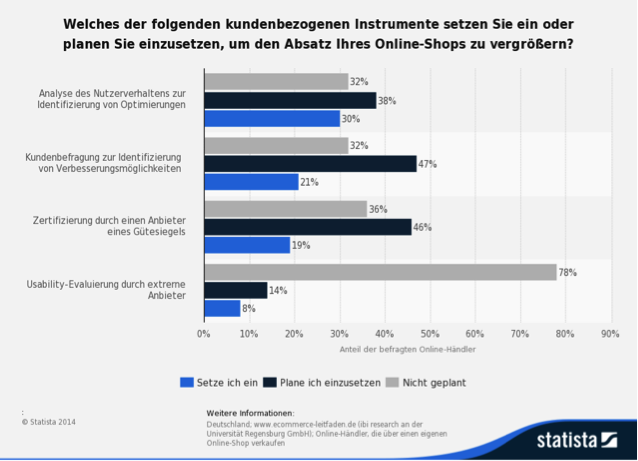
\includegraphics[width=\textwidth]{figures/Roesener2.png}
 \caption{Instruments to improve the sales of online shops (Source: ibi research University Regensburg GmbH 2014)}
 \label{roesener:fig:2}
\end{figure} 



The results show clearly that, despite the problem shown in \figref{roesener:fig:1}, very few online retailer actually use (8\%) or plan to use (14\%) usability engineering to improve their web sites. With these two statistics alone, the large potential of usability engineering and research becomes clear. These findings can therefore well serve as a motivation to design and create a contemporary usability lab.

\subsection{Methods and techniques}

To achieve the abovementioned goal ``to measure the quality of the user experience'', various research methods and techniques exist:

\begin{itemize}
\item observation
\item pre- and post-test questionnaires 
\item (retrospective) interviews 
\item paper prototyping 
\item co-discovery learning, etc.
\item think-aloud protocols 
\item keyboard and mouse logging 
\item video and audio recording, etc. 
\end{itemize}

Furthermore, in addition to all the methods and techniques above, eye tracking is a key research method conducted in every usability laboratory. So, on the one hand a contemporary usability laboratory should provide the latest eye tracking equipment. On the other hand, all of the abovementioned methods and techniques for usability research should also be technically supported.

\subsection{Starting point}

At Flensburg University of Applied Sciences, eye tracking research was planned mainly in two scientific fields. One was eye tracking for language and translation research, i.e. research concerning reading behaviour, gaze pattern analysis and the comprehensibility of texts \citep{Hennig2007}. The other field was eye tracking for usability engineering, i.e. to analyze, test and evaluate software interfaces (especially of language and translation software) \citep{HansenSchirra2013}, to test and evaluate online manuals and online help in technical communication (especially on mobile devices), to investigate operation of machinery (operating cycles, work processes), to analyze, test and evaluate web and software interfaces in other areas (for example, mechanical and electrical engineering). Furthermore, for future projects research concerning industrial design and design rationale respectively were envisioned.


It was thus very clear that eye tracking should serve two purposes in the future usability laboratory at Flensburg University of Applied Sciences: as a key research method for language and translation research as well as a key research method for usability testing. That meant that these two different approaches had to be implemented in the same laboratory. This in turn had a significant impact on the choice of which equipment and software systems to purchase and on the laboratory design.


\section{Eye tracking and usability engineering }

\subsection{Eye tracking systems -- spoilt for choice }

The first problem to deal with when implementing a contemporary usability laboratory is the manifold variety of technical equipment, especially concerning the eye tracking equipment. Holmqvist states that ``in 2009 we found 23 companies selling video based eye tracking systems'' \citep[12]{Holmqvist2011}. In my view, however, there are only a small number of traditional manufacturers providing equipment for academic research\footnote{ This selection is clearly subjective. However, it is definitely not the intention of the author to favour certain manufacturers. The selection is based on the author's experience and on discussions with colleagues working in other existing language and translation research eye tracking and/or usability laboratories. Thus, the list makes no claims of being complete.}: 

\begin{itemize}
\item ASL -- Applied Science Laboratories, Bedford, USA
\item SMI -- Sensomotoric Instruments, Teltow, Deutschland
\item SR-Research, EyeLink System, Ottawa, Kanada
\item Tobii, Danderyd, Sweden 
\end{itemize}


Of course, there are many more new competitors, like, for example, Mangold International GmbH, Arnstorf, Interactive Minds GmbH, Dresden, both Germany and Eyetech, Digital Systems, Mesa, USA to name but a few. However, these manufacturers in my opinion offer equipment more for media and advertisement consultants than for profound scientific research. Besides the manufacturer, the final buying decision should mainly be based on two questions: ``What do I really need?'' and ``Which manufacturers meet my requirements?'' The first decision that has to be taken is about which of the eye tracking working solutions are required for the planned laboratory. Basically, there are three different types of eye tracking systems: workstations, mobile solutions and eye tracking glasses. In \figref{roesener:fig:3} an example of each solution is given.


 
\begin{figure}[t]
 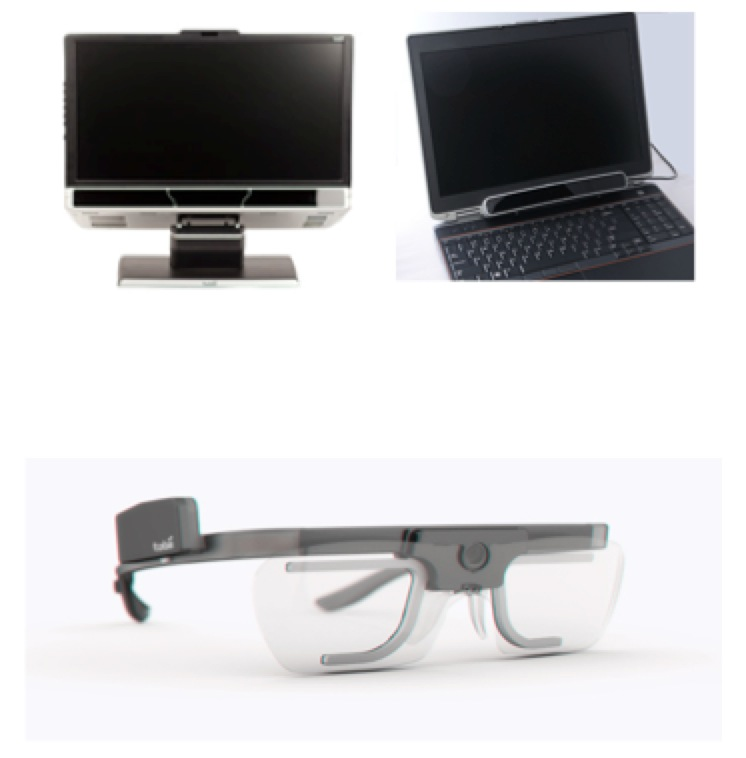
\includegraphics[width=\textwidth]{figures/Roesener3.png}
 \caption{Eye tracking workstation, mobile eye tracker, eye-tracking glasses (Tobii 2014 / SMI 2014)}
 \label{roesener:fig:3}
\end{figure} 


As the name implies, mobile eye tracking solutions are designed for research in varying environments, for example, on-site research with laptops in companies. Eye tracking workstations on the other hand are laboratory-based and deliver the most accurate results. Finally, eye tracking glasses are suitable for fully mobile eye tracking studies, for example, operating machinery.


Additionally, there are a lot of properties to consider when purchasing an eye tracking system for a usability laboratory. At this point, I will briefly discuss only three main issues, which again in my view are very important for the final decision regarding which manufacturer to choose and which solution to buy: the sampling rate, the different solutions for testing mobile devices and the system license policy of each manufacturer. Other relevant parameters for comparison might be mobility, handling, workmanship, software features and of course price, to name but a few. 



The decision to discuss only the three abovementioned issues was taken for the following reasons: The sampling rate is of major interest especially when planning to do language and translation research in the usability lab, because when investigating reading behaviour or comprehensibility of texts, for example, you have to deal with very rapid eye movements. The solutions for testing mobile devices are taken into account because more and more mobile devices, instead of stationary computers, are used for tasks like reading texts, editing texts and so on. From the point of language research, that makes this issue very important for the design of a future-oriented usability laboratory. And finally, the systems license policy is chosen as an issue because it is very difficult within public institutions like universities to achieve long term financing for projects or equipment. Therefore, the license terms and conditions of the manufacturers are of major importance to achieving a sustainable long term solution for the planned usability laboratory.


\subsubsection{Sampling rate}

As noted by \citet[29]{Holmqvist2011} ``[t]he sampling frequency is one of the most highlighted properties of eye trackers by manufacturers, and there is a certain competition in having the fastest system.'' The sampling rate is measured in Hertz (Hz = times per second) and various systems with sampling rates from 25-30 Hz up to more than 1000 Hz do exist. Reasons for not purchasing a fast system can be that high-speed eye trackers are more expensive, that they are more restrictive to the participants and that they produce larger data files. On the other hand, a high sampling rate is necessary for certain eye tracking measures as shown in \figref{roesener:fig:4}.

\begin{figure}
 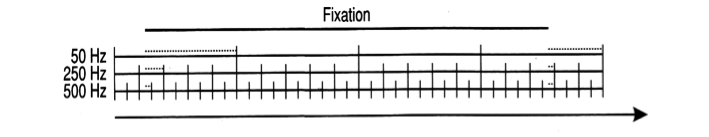
\includegraphics[width=\textwidth]{figures/Roesener4.png}
 \caption{Fixation recorded at different sampling frequencies \citep[31]{Holmqvist2011}}
 \label{roesener:fig:4}
\end{figure} 


On top of \figref{roesener:fig:4}, you have a fixation of a certain time shown as solid line. Along the timeline of the figure, each small peg stands for a photo of the eye. Then the gaze position is calculated and a sample is recorded. The errors -- indicated with dashed lines in the figure -- are much larger for slower systems. Of course, there are also other eye tracker specific properties for data quality, for example, latency (saccadic latency, saccadic velocity and acceleration) as well as accuracy and precision. However, the decision which system to purchase depends first of all on the question of what you need to detect or measure. It can be stated that the faster the eye movement you want to analyse the faster your system and the sampling rate respectively has to be. For more information about the influence of the sampling rate on eye tracking research setup and results see Andersson \citep[cf.][]{Andersson2009}. 

\subsubsection{Testing mobile devices}

As shown in \figref{roesener:fig:5} different manufacturers offer various solutions for testing mobile devices. 

\begin{figure}
 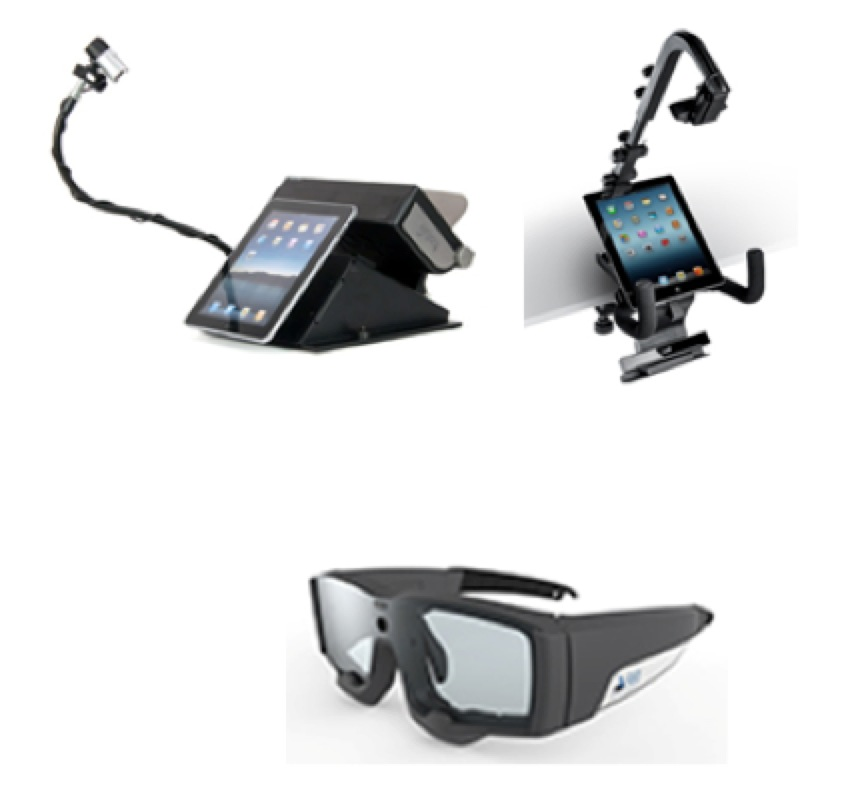
\includegraphics[width=\textwidth]{figures/Roesener5.png}
 \caption{Mobile device stands and eye tracking glasses \citep{Tobii2014, SMI2014}}
 \label{roesener:fig:5}
\end{figure} 

For testing of mobile devices, so called mobile device stands (MDS) as well as eye tracking glasses are suitable. However, each solution has its advantages and disadvantages. Mobile device stands provide a very accurate analysis of small design elements, because the mobile device is always fixed in the stand and thus the data recording is of better quality. Eye tracking glasses will definitely not deliver the same data quality. On the other hand, the participant-device interaction is unnatural with mobile device stands. As illustrated in \figref{roesener:fig:5}, both MDS solutions fix the mobile device. Even worse, between the two rods of the MDS, shown on the right side in \figref{roesener:fig:5}, no movement of hands is possible, because as the eye tracker is mounted underneath the mobile device, any movement of the hands here would make eye tracking impossible.


On the other hand, eye tracking glasses can be used very flexibly. The glasses can be worn almost like ordinary glasses. Thus, a natural participant-device interaction is guaranteed, as you can use the glasses in day-to-day situations, for example, using a tablet computer in an armchair. As a result, a HD video of the field of view is recorded, with a point indicating where the participant looks. The only disadvantage of that setting might be that with the eye tracking glasses the analysis of small design elements is not of the same quality as with a MDS. Again the decision which solution to choose depends on the research preferences.


\subsubsection{System license policy}

Another last important point to consider when purchasing software for an eye tracking or usability laboratory is the system license policy of each manufacturer. Here significant differences do exist, which can be crucial for the final decision. Especially the following conditions have to be taken very carefully into account:

\begin{itemize}
\item purchase or rental 
\item support and updates 
\item upgrade cycles and method 
\item various software packages for different tasks 
\item network licenses (work with student groups)
\end{itemize}


The decision whether to buy or rent a software system is often influenced by the administration of the universities. Usually -- especially within project funding -- the universities prefer one-time instead of regular payments. Therefore, a rental solution is often out of question. In addition, the support and future updates should be included in the purchase. Some manufacturers offer only fee-based support and updates, which is again difficult to realize within projects. It is also very important to know, whether the offered support is gradual and, if yes, which support I will get with the planned purchase.


Finally, also the type of support (ticket system, etc.), office hours and response time should be considered, as well as the upgrade cycles and method. A complicated upgrade method can be annoying and very time consuming and should be avoided for that reason. To take a closer look on the software packages offered is also recommended. It is very important that the eye tracking software allows one to analyze collected data on different computers, so that it is possible to work with groups of students. Additionally, for a convenient research and teaching situation, it should be possible to run several software systems at the same time, so that analyzing data on several computers in a pc network with groups of students becomes possible.


\subsection{Deploying a usability laboratory to serve all interests -- the Swiss army knife }

When deploying a usability laboratory, one of the most difficult tasks to fulfil is to serve the different interests of the future users of the laboratory. All the different research areas have to be taken into account, especially when a broad multidisciplinary use of the laboratory is planned. First of all, for eye tracking for language and translation research it is necessary that the eye tracking equipment operates at a high sampling rate. Only this enables research in the area of reading behaviour, gaze pattern analysis and comprehensibility of texts. To serve this research interest the purchase of an eye tracking workstation is mandatory.


On the other hand, usability engineering requires mobile solutions for eye tracking. Here a high sampling rate is not as important as the mobile aspect. Usability research should be possible not only in the laboratory but also in natural participant-device interaction in day-to-day situations outside the usability lab. Therefore, mobile eye tracking solutions as well as eye tracking glasses are needed. Only with this equipment is it possible to do, for example, on-site research of operation of machinery and web and software interfaces. 



Additionally, usability engineering requires further equipment of the laboratory as well. For example, video cameras and microphones, several video screens and special usability software to process the collected data (e.g. `Morae' from TechSmith) are necessary to conduct research not only in the area of software interfaces and human computer interaction, but especially in the area of industrial design and design rationale. The main focus in this field is user observation, interviews and think aloud protocols. To conduct this kind of research video and audio equipment as well as special user experience and market research software is needed. Moreover, when it is planned to combine results from electroencephalography (EEG) recordings with the usability testing, the laboratory needs to be equipped with a brain computer interface or EEG system respectively. And of course, all software systems should work together, i.e. have common interfaces so that recorded data can be exchanged without any problems.



The same applies to experimental design and setup. If research is planned and conducted in all the abovementioned fields, the laboratory should be suitable for all possible different experimental designs and setups, which means there should be enough space for equipment, participants and test objects in the laboratory. To fulfill these requirements at least two rooms -- one laboratory (test room) and one observation room, separated by a wall with a one way mirror -- are necessary. \figref{roesener:fig:6} shows a possible layout of a usability laboratory.



Of course, several layouts for usability laboratories are possible. For example, the `executive observation lounge' in \figref{roesener:fig:6} is not essential for running a successful usability laboratory. It might be interesting though for a third group of observers to discuss the test without disturbing the experimenters and usability specialists in the observation room \citep[cf.][203ff.]{nielsen1993}. In my view for academic purposes, the one laboratory solution is absolutely sufficient. Naturally, if larger groups or a lot of participants should be tested simultaneously a multi-laboratory solution would be appropriate. However, this applies rather for bigger companies, where series of tests with large groups are conducted.


\begin{figure}
 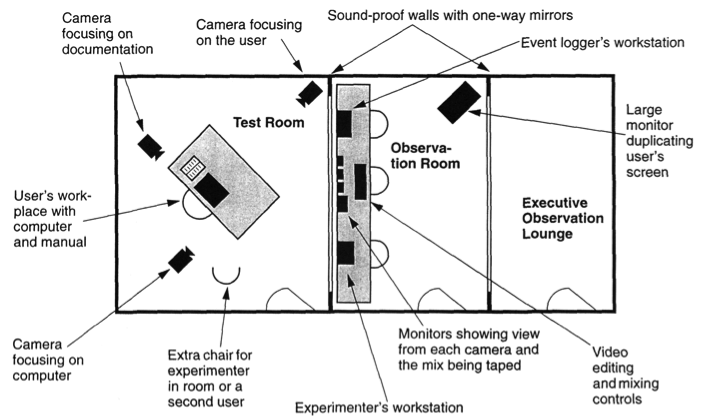
\includegraphics[width=\textwidth]{figures/Roesener6.png}
 \caption{Floor plan for a hypothetical usability laboratory \citep[201]{nielsen1993}}
 \label{roesener:fig:6}
\end{figure} 


In addition to the room or space problem, there are many other necessary properties of the recording environment, which have to be considered when developing a contemporary usability laboratory. It would be far too much to list all possible circumstances, which can cause problems for the experimental setup or lower the quality of the data recorded in the usability lab. Nevertheless, I want to point out a few conditions, which are important in my opinion and easy to consider in order to avoid problems before or during usability tests. Cramped recording space, for example, makes it uncomfortable for the participants to attend usability experiments. Therefore, you have to make sure that the participants themselves feel comfortable before and during the actual usability tests. One precondition to achieve this is enough room space. The lab should be spacious enough so that the participants do not feel cramped. Lab availability correlates with that. If the lab is only available in very restricted times, it becomes very difficult to get the participants to show up. Regular working hours of the usability laboratory help to counter this problem.


 Sunlight in the laboratory is another problem. It can affect eye tracking experiments by creating optic artifacts and imprecision. Of course, you can dim the laboratory with sun blinds, but the best solution for a usability laboratory is to have either windows to the north, so that sunlight never shines into the lab, or no windows at all, at least in the test room. Another problem connected with this is lamps and lighting conditions in general. Depending on how and which lamps are positioned under the ceiling in relation to the eye tracking equipment this might also cause imprecision as well as optic artifacts. The best solution is to use neon light instead of light bulbs or halogen lamps, and to create lighting conditions in the usability laboratory, which can be changed manually, for example, with dimmer controlled lamps and electrically adjustable shades.



It is also advisable to minimize various sources of electromagnetic noise. In order to avoid inaccuracy, low precision or -- in the worst case -- data loss try to locate your usability laboratory away from lifts and ban fans and other electronic equipment causing electromagnetic noise from your usability lab as well as from the neighbouring rooms. The same applies for vibrations and noise. Try to avoid people moving nearby as well as noise and vibrations caused by outside traffic. This can seriously affect your data quality. It is therefore advisable to use a soundproof room. However, this is often impossible for financial reasons.


\subsection{The dos and don'ts -- the most common mistakes }

Concerning the dos and don'ts in the process of developing and implementing a contemporary usability laboratory there are -- in my view -- two main areas of most common mistakes: theoretical mistakes and practical mistakes. The most common theoretical mistakes to mention, when starting to develop the idea of a usability laboratory, are mistakes concerning the imagination of experiment design and experimental setup. Most of the time, the future users of a usability laboratory have a very good idea of what they want to test or analyze. But they have not thought about what exactly they want to know or investigate. To take one example, the idea is to test the comprehensibility and the usage of machine operating manuals. But what exactly should the test scenario be and what kind of results should test which assumption is not clear at all. 


In a lot of these cases the eye tracking or usability equipment is purchased before the experiment design and the experimental setup is well conceived. Quite often future users have not thought about what kind of results they want to achieve, when the order for the equipment is placed. And because of this, after a while, it becomes clear that certain equipment, additional software or other preconditions, which would be necessary to conduct specific experiments, have not been foreseen or ordered in the process of the implementation of the laboratory. This can lead to a significant level of frustration and -- even worse -- to the situation that a brand new usability laboratory is then no longer used by the initially very interested user groups, because their expectations could not be fulfilled. Do not expect especially the experimental setup to be easy. It is worthwhile to sit together with all interested future user groups and discuss and develop a detailed plan, what kind of experimental setup each different user plans to realize in the lab, before you start the implementation of the new usability laboratory and before you order the equipment and software systems respectively.



The most common practical mistakes happen when the usability laboratory is already implemented and running. Quite often, the optimistic expectations of the new users are very soon disappointed when they start their first experiments in the new lab. Out of the manifold difficulties, which may occur, once you get started with usability experiments, I would like to point out a few general problems here, which can cause immediate frustration and disappointment. A big problem, for example, are eye tracking experiments with wearers of glasses or contact lenses. This is something new users should be absolutely aware of. It is very difficult, if not impossible, to conduct experiments and/or to get high quality eye tracking data from experiments with wearers of glasses or contact lenses. This is particularly interesting because the manufacturers are quite reserved about this fact and talk rather hesitantly, if at all, about it. Definitely, in experiments with wearers of glasses or contact lenses more problems than expected will occur. Some of the manufacturers encounter this problem providing corrective lenses at least for the eye tracking glasses. Nevertheless, the problem persists with stationary and mobile eye trackers.



Another point is the adjustment or configuration of the system. At the beginning, quite often users do not pay much attention to the adjustment or configuration of the eye tracking equipment and the software respectively. And then they are disappointed when the results they get are not of very good quality. Here again, it is worthwhile to spend some time with an initial training how to adjust and configure the system. The better the configuration and the adjustment of the system, the better the quality of the data finally recorded.



Despite these two main points, there are a lot of other factors which influence the quality of the recorded eye tracking data. For example, the fact that all participants are different concerning nose size, head form, distance between the eyes, etc. requires a very careful experimental setup. Some of the manufacturers try to encounter several of these problems by providing, for example, different types of nose rests, adjustable glasses and special software possibilities. However, that helps only to a certain extent. The common practical mistake is too little time spent to do the setup of the system very carefully. The same applies for the furniture of the actual test or observation room. An important point here is the types of chairs for the participants. Make sure that no swivel chairs are used. These chairs make the participants move more than necessary and thus cause bad data quality. For the same reason the chairs should not have adjustable armrests nor adjustable back or seating surfaces. All this causes bad data quality or even loss of data. The table for the eye tracking workstation is another sensitive point. Due to the various heights of the participants, the monitor and the eye tracker have to be adjusted each time in its horizontal position to fit the respective person. To prevent damage to the monitor and the eye tracker respectively because of this frequent adjustment, it is recommended to use an electrically controlled height-adjustable table instead. It is comfortable to use and damage to the eye tracking equipment or the monitor can be easily avoided. However, the most common mistake when developing and implementing a new usability laboratory is that the expectations of the users are often pitched far too high. Quite often too much is expected from the technology alone. 


\subsection{The usability laboratory at Flensburg University of Applied Sciences -- an attempt }

At Flensburg University of Applied Sciences, the new usability laboratory consists of two rooms. The observation room/control room size is about 11 m² and the actual test room/usability recording studio size is about 23 m². The rooms are separated by a wall with an inbuilt one way mirror. The floor plan/layout of the actual usability laboratory is shown in \figref{roesener:fig:7}. 


There are two video cameras in the laboratory. The cameras are mounted under the ceiling in opposite corners of the test room/recording studio. Together with additional microphones, it is possible to record both audio and video data from the test room. Focused on the user and on the computer screen or documentation the cameras provide two video views, which can be mixed together with special software in the observation room/control room. 



The usability laboratory at Flensburg University of Applied Sciences is an example for a compromise between an eye tracking laboratory for language and translation research only on the one hand and a fully equipped usability lab on the other hand. It combines features and possibilities of both worlds so that it serves most of the interests of the different future user groups. 


\begin{figure}
 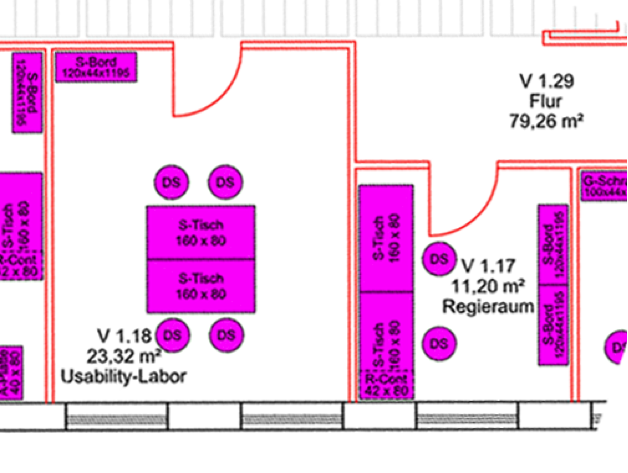
\includegraphics[width=.8\textwidth]{figures/Roesener7.png} 

 \caption{Floor plan / layout of the usability laboratory of Flensburg University of Applied Sciences (test room and small control room; separating wall with one way mirror)
}
 \label{roesener:fig:7}
\end{figure} 


\section{Conclusion and outlook }


Looking back at the process of planning, creating and implementing a contemporary usability laboratory at Flensburg University of Applied Sciences, I want to draw some key conclusions on the whole effort as well as to give some prospects about the desired possible future activities. The idea of developing a usability laboratory at Flensburg University of Applied Sciences came about two years ago. Based on an interdisciplinary cooperation between three courses of study, the course of study International Technical Communication, the course of study Applied Computer Science and the course of study Media Informatics, an initiative was launched to make an application to the Ministry of Education of Schleswig-Holstein for funding a human computer interaction and usability laboratory. When the funding was finally granted, a group of people started to work out a development plan and a roadmap for the two laboratories.



From the beginning, the plan was to use the usability laboratory not only within one single study course. On the contrary, it was clear from the start that the future usability laboratory has to provide research opportunities for usability engineering in general and eye tracking research in particular. Therefore, the persons involved in the development of the future usability laboratory were truly aware of the necessity to purchase not only eye tracking equipment. Nevertheless it was, even at this stage, difficult to meet all the requirements of the various interested user groups. Besides the so called `language people', who were interested in language and translation research (reading behaviour, gaze pattern analysis and comprehensibility of texts, etc.), there were a lot of other people with different research interests: people from the department of economics, who wanted to do market research; people from the department of education of Flensburg University, who wanted to do gaze pattern analysis in picture reception; people from the department of mechanical engineering, who wanted to do research concerning the operating of machinery and so on and so forth. It soon became very clear that it was extremely difficult do meet all the existing demands of the different parties involved.



To solve this problem, the next step in planning the new usability laboratory was to collect the various ideas and research interests of the different future user groups and departments and transfer them into realistic experiment setup and experimental design respectively. This turned out to be very difficult as well. First of all, it was very difficult to really identify the demand of some interest groups. Some of the parties involved had only a very vague imagination about what they really wanted to do. Most of the time the problem was that they were not or only to some extent familiar with the subject of usability engineering or eye tracking research in general. So, already at this point, it is really necessary in the process that the people involved have some knowledge about the different techniques and methods used in usability engineering. 



The second problem was to transfer the existing demands into real experimental design and setup. This requires also, even at this stage of the process, detailed knowledge about the possibilities of the different equipment and systems. Of course, this applies only for a smaller group of people, who are finally involved in placing the order for the equipment and software systems respectively. But it is nevertheless very important that these people have detailed knowledge about the potential and possibilities of various equipment and software systems. 



At this point, I would like to mention another very interesting fact about the manufacturers of eye tracking equipment and systems. During the process of creating and implementing the usability laboratory at Flensburg University of Applied Sciences, we had the experience that some manufacturers are very accommodating when it comes to discounts for universities. Some manufactures offer significant discounts for eye tracking equipment and software systems. The offers quite often come in the form of bundle software and hardware packages or as `educational licenses', etc. Analyzing the sales policy of the relevant manufacturers can really save a lot of money in this context.


\subsection{Recommendations}

From the `lessons learnt' point of view I would like to make some recommendations on the basis of which -- in my view -- a lot of problems can be avoided when implementing a contemporary usability laboratory, which should serve -- in the best possible way -- all research interests of the different parties and interest groups. It is extremely important to involve all possible future user groups in the planning already from the beginning. So, the first step in the process of developing a usability laboratory has to be the analysis of the situation at your university or institution. Ask the different parties and possible future user groups what kind of research they want to conduct in the planned laboratory. On this basis then clear experimental setups and designs should be developed. All this should be done before ordering the equipment, because it is very difficult, time consuming and annoying to cancel or change orders once they are placed. It is definitely much better to know what equipment and system is suitable to meet your special requirements. `One step at a time' is the best strategy when planning and implementing a usability laboratory.


For the implementation and operation of a contemporary usability laboratory also keep in mind that technology is only as good as the people who use it. So again, from the beginning when you plan your resources you have to make sure that you have the staff to operate the laboratory in a proper way. Do not expect too much from the technology alone. A usability laboratory can not be operated without the appropriate staff. The administration and management of the laboratory when working with participants or whole user groups as well as the handling of the equipment and software systems require qualified and competent personnel. Moreover, in some cases it might even be necessary to have personnel to programme additional software to run certain experiments or analyse recorded data. Furthermore, if you intend to provide regular laboratory opening hours, appropriate staff will also be required. 


\subsection{Outlook}

A sustainable implementation of any contemporary usability laboratory at a university or similar institution is -- in my opinion -- only possible if a few key principles are observed. These principles are multiplicity, integration, expertise and self determined learning. Multiplicity in this case simply means that the usability laboratory should be used by many different users and groups, for example, various courses of study from different departments and faculties. Thereby a high acceptance and recognition of the subject usability is ensured. Integration on the other hand guarantees for permanent utilization of the laboratory. If usability engineering becomes a proper component of teaching and research activities of several courses of study, the laboratory will be permanently in use. In addition, growing usability engineering expertise due to many interdisciplinary projects will lead to a more effective usage of the laboratory, and subsequently also to better (project) results.


Finally, student projects, based on self-determined learning principles and with the usability laboratory involved in the research, create a very attractive field of studies. Once the students start to develop their own research projects and conduct their own eye tracking or usability tests in the laboratory, usability engineering is well established as an attractive field of research in the courses of study. This could then, due to project papers and bachelor and master theses, lead to more ``usability driven'' contacts with companies and manufacturers on the market. And this in turn guarantees that the courses of study offered at the university are vocationally orientated and of high practical relevance. All the abovementioned points apply especially for Flensburg University of Applied Science. The full integration of the new usability laboratory into teaching and research activities of the university is the main objective and the desirable future for this laboratory.


% \section{References}
% 
% 
% Andersson, Richard / Holmqvist, Kenneth / Nyström, Marcus. 2009/2010. “Sampling frequency and eye-tracking measures: how speed affects durations, latencies, and more“. Journal of eye movement research. 3(3), 6, 1-12. Available online: http://www.jemr.org/online/3/3/6
% 
% 
% 
% \emph{Dumas, Joseph S. / Redish, Janice C. 1999. }“A Practical Guide To Usability Testing. “ Revised Edition, Intellect Books: Exeter. United Kingdom.
% 
% 
% 
% Hansen-Schirra, S. / Rösener, C. 2013. “Proactive Use of Eye-Tracking in the Translational Workflow. “ In Translation Studies and Eye-Tracking Analysis, edited by S. Grucza, M. Pluzyczka and J. Zajac. , J.: Translation Studies and Eye-Tracking Analysis. In Druck: Peter Lang 2013.
% 
% 
% 
% Eichinger. A. (1999). “Usability“. Script of the department of psychology II of Regensburg University. http://pc1521.psychologie.uni-regensburg.de/ student 2001 / Skripten/Zimmer/usability.html
% 
% 
% 
% Hennig, Jörg / Tjarks-Sobhani, Marita (Hg.). 2007. “Usability und Technische Dokumentation. “ Lübeck: Schmidt-Römhild. Lübeck. Germany.
% 
% 
% 
% Holmqvist, Kenneth / Nyström, Marcus et. al. 2011. “Eye Tracking. A comprehensive guide to methods an measures.“ Oxford University Press: Oxford. United Kingdom.
% 
% 
% 
% ISO 9241. 1992. “Ergonomic requirements for office work with visual display terminals“. From 2006 "Ergonomics of Human System Interaction". International Organization for Standardization. Geneva. Switzerland.
% 
% 
% 
% Nielsen, Jakob. 1993. “Usability engineering“. Morgan Kaufmann; New edition (11th November 1994). Amsterdam. Netherlands.
% 
% 
% 
% Nielsen, Jakob. 1998. “The Increasing Conservatism of Web Users“. Online: http:// www.useit.com/alertbox/980322.html
% 
% 
% 
% SMI. 2014. Website: http://www.smivision.com – 22nd September 2014
% 
% 
% 
% Tobii. 2014. Website: http://www.tobii.com – 22nd September 2014



%\subsection*{Abbreviations}
%\subsection*{Acknowledgements}

{\sloppy
\printbibliography[heading=subbibliography,notkeyword=this]
}
\end{document}